% PLANTILLA APA7
% Creado por: Isaac Palma Medina
% Última actualización: 25/07/2021
% @COPYLEFT

% Fuentes consultadas (todos los derechos reservados):  
% Normas APA. (2019). Guía Normas APA. https://normas-apa.org/wp-content/uploads/Guia-Normas-APA-7ma-edicion.pdf
% Tecnológico de Costa Rica [Richmond]. (2020, 16 abril). LaTeX desde cero con Overleaf (1 de 3) [Vídeo]. YouTube. https://www.youtube.com/watch?v=kM1KvHVuaTY Weiss, D. (2021). 
% Formatting documents in APA style (7th Edition) with the apa7 LATEX class. https://ctan.math.washington.edu/tex-archive/macros/latex/contrib/apa7/apa7.pdf @COPYLEFT

%+-+-+-+-++-+-+-+-+-+-+-+-+-++-+-+-+-+-+-+-+-+-+-+-+-+-+-+-+-+-++-+-+-+-+-+-+-+-+-+

% Preámbulo
\documentclass[stu, 12pt, letterpaper, donotrepeattitle, floatsintext, natbib, helv]{apa7}
\usepackage[utf8]{inputenc}
\usepackage{comment}
\usepackage{marvosym}
\usepackage{graphicx}
\usepackage{float}
\usepackage[normalem]{ulem}
\usepackage[spanish]{babel} 
%\usepackage{titling}
\let\apasubparagraph\subparagraph
\let\subparagraph\paragraph
\usepackage[compact]{titlesec}
\let\subparagraph\apasubparagraph
\usepackage{hyperref}
\selectlanguage{spanish}
\useunder{\uline}{\ul}{}
\newcommand{\myparagraph}[1]{\paragraph{#1}\mbox{}\\}
\graphicspath{{./images/}}
\titleformat{\section}{\normalfont\large\bfseries}{\thetitle. \quad }{0pt}{}[{ \titlerule[0.8pt]}]
\titleformat{\subsection}{\normalfont\bfseries}{}{}{}[]

% Portada

\begin{document}
\begin{titlepage}
    \centering
    \vfill
    \LARGE Laboratorio \#2\\
    \vskip2cm
    \large Diego Quirós Artiñano \\
    Universidad Nacional de Costa Rica \\
    EIF-202: Soporte Técnico \\ 
    Carolina Gómez Fernández \\
    27 de marzo, 2022 \\
    \vfill
    
\includegraphics[width = 0.4\textwidth]{../../../UNAImage/UNA.png} \\
    \vfill
    \vfill
    % (autores separados, consultar al docente)
    % Manera oficial de colocar los autores:
    %\author{Autor(a) I, Autor(a) II, Autor(a) III, Autor(a) X}
\end{titlepage}

% Índices
\pagenumbering{roman}
    % Contenido
\renewcommand\contentsname{\largeÍndice}
\tableofcontents
\setcounter{tocdepth}{2}
\newpage
    % Figuras
\renewcommand{\listfigurename}{\largeÍndice de fíguras}
\listoffigures
\newpage
    % Tablas
%\renewcommand{\listtablename}{\largeÍndice de tablas}
%\listoftables
%\newpage

% Cuerpo
\pagenumbering{arabic}

%------------------------------------------------------------------------------------
\section{Introducción}
En este laboratorio se van a solucionar problemas de circuitos usando Arduinos y se va a concretar conocimientos desconocidos haciendo un glosario de palabras desconocidas.

%------------------------------------------------------------------------------------
\section{Parte 1 Ejercicios de Arduinos}
Para ver las soluciones de los ejercicios en tinkercad ver referencias. \cite{tinkercadEjercicios}

\begin{figure}[h]
    \centering
    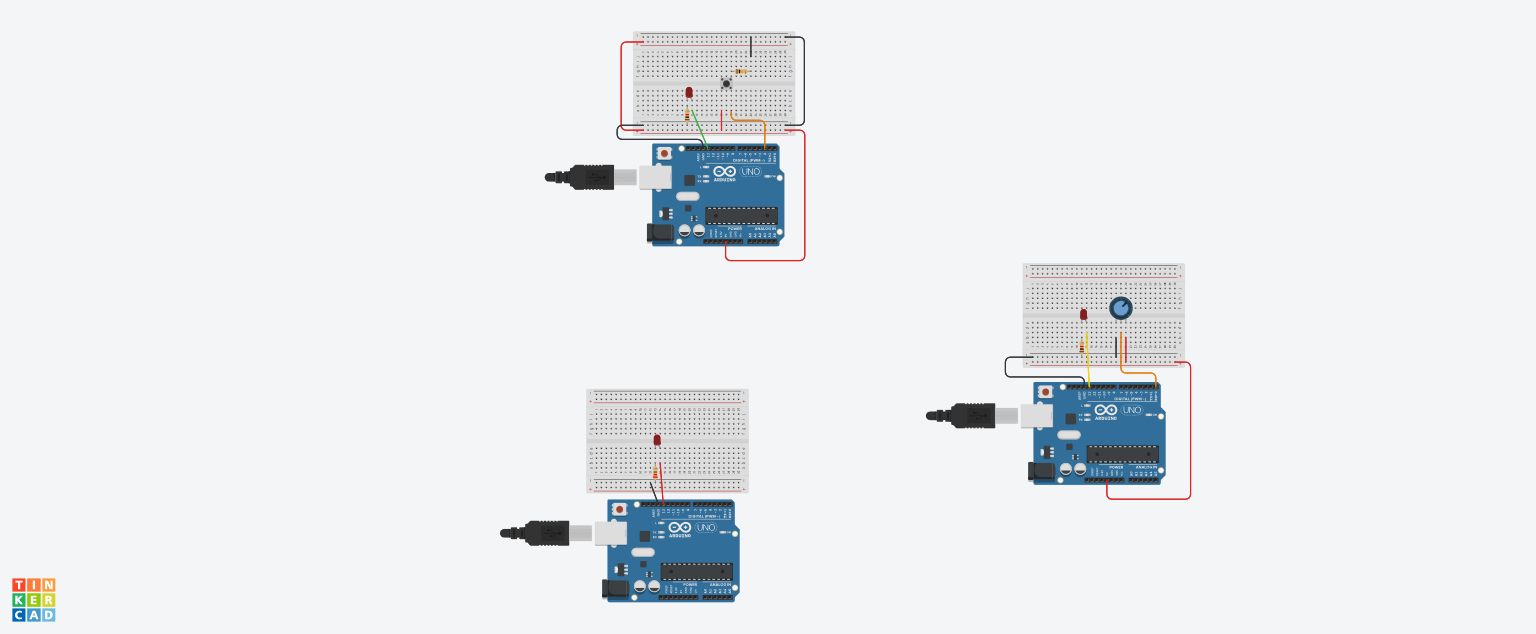
\includegraphics[width=1\textwidth]{Lab2Exercises.png}
    \caption{Imagen de los ejercicios de Tinkercad}
    \label{fig:figArduinos}
\end{figure}

%----------------------------------------------------------------------------------------------------------------------------------
\section{Parte 2 Glosario de palabras desconocidas}
Yo ya tenía experiencia con Arduinos del colegio entonces no son muchos los términos que no entiendo, pero finalmente me hizo click algunas cosas por la electrónica digital/analógica

\begin{itemize}
    \item El digitalRead(pin) (conclusión basada en el video de la semana pasada: \cite{video}) se define así porque la electrónica digital es como subir una escalera, no se puede medio escalón.
    \item El analogRead(pin) (conclusión basada en el video de la semana pasada: \cite{video}) se define así porque los valores que obtiene este es de electrónica analógica y si puede tener "medio escalones".
    \item Potenciómetro: (aunque ya haya trabajado nunca concreté una definición específica para este), según la Real Academia Española (\cite{potenciometroDef}) es un \begin{quoting} Instrumento que mide las diferencias de potencial eléctrico \end{quoting}, el cuál tiene sentido de la manera en la que lo usamos y mi experiencia prueba y además concuerda con la idea de electrónica analógica.
\end{itemize}

%----------------------------------------------------------------------------------------------------------------------------------------------------------------------
\section{Conclusión}
En este documento se hicieron ejercicios de circuitos con Arduinos, esto ayudó a cementar la idea e implementación de un circuito, sea con interruptores o no, y haciendo de una manera para que tampoco se queme nada. En este laboratorio también se siguió investigando sobre elementos que no conocíamos sobre el tema, esto no solo ayuda con el auto-aprendizaje, sino que también a fomentar curiosidad y conocimiento en el área. En mi caso logré implementar el conocimiento del laboratorio pasado y entender algunas cosas que ya medio había traveseado.

\newpage
% Referencias
\renewcommand\refname{\large\textbf{Referencias}}
\bibliography{ref}

\end{document}